\section{Differential Calculus in $\mathbb{R}^d$}

\subsection{Stetigkeit (Continuity)}

Definition Stetigkeit:

\[
    \lim_{x\rightarrow x_0} f(x) = f(x_0)
\]

Definition Stetigkeit mit Folgen: Für jede Folge $(x_n)$ sodass $x_n \rightarrow x$ für $x\rightarrow \infty $:

\[
    (f(x_n)) \rightarrow f(x)
\]

Mit $f,g$ stetig: $f+g$, $f\cdot g$, $\frac{f}{g}$, $f \circ g$ stetig.

Falls $f$ stetig, gilt

\[
    \lim_{x \rightarrow a} f(x) = f(\lim_{x\rightarrow a} x)
\]

$f$ diffbar $\Rightarrow$ $f$ stetig $\Rightarrow$ $f$ integrierbar

$f$ nicht integrierbar $\Rightarrow$ $f$ nicht stetig $\Rightarrow$ $f$ nicht diffbar.\\

\textbf{Polarkoordinatentrick (change of variable, coordinates)} (um Stetigkeit zu beweisen oder widerlegen) Let $x=r\cos \varphi$, $y=r\sin \varphi$. Berechne

\[
    \lim_{(x, y) \rightarrow (0,0)} f(x, y) = \lim_{r \rightarrow 0} f(x, y)
\]

Das Resultat hängt von $\varphi$ ab $\Rightarrow$ der Grenzwert existiert nicht $\Rightarrow$ nicht stetig an dieser Stelle.\\

\textbf{Linientrick} (um Stetigkeit zu widerlegen): Suche zwei Linien, die einen unterschiedlichen $\lim$ haben. Zeigt, dass ein $\lim$ nicht existieren kann.
Let $f(x, y)=\frac{y}{x+1}$ und $\{(x, y) \in \mathbb{R} \mid x \neq 1\}$ für $(x, y) \rightarrow (-1, 0)$. Linie $\{(x, y) \in \mathbb{R} \mid y=0\cap x \neq 1\}=0$ und $\{(x, y) \in \mathbb{R} \mid y=x+1\}=1$.\\

\textbf{Rezept Stetigkeit prüfen}: 1) $f$ muss überall definiert sein. 2) $\lim_{x \rightarrow a} f(x)$ existiert. 3) $\lim_{x \rightarrow a} f(x) = f(a)$.

\subsection{Differenzierbarkeit (Differentiable)}

$f$ diffbar $\Leftrightarrow$ alle Teil-$f$ sind diffbar.

$f,g$ diffbar $\Rightarrow$ $f+g$, $f \cdot g$, $\frac{f}{g}$, $g \circ f$ diffbar

TODO: skript proposition 3.4.4

TODO: regeln differenzierbarkeit: addition, multiplikation, division, verkettung (proposition 3.4.9)

TODO: tangent space of $f$

\textbf{Partielle Differenzierbarkeit}: $f$: $\mathbb{R}^n \rightarrow \mathbb{R}^m$, falls:

\[
    \lim_{h \rightarrow 0} \frac{f(x_0 + h e_i)-f(x_0)}{h} =: \frac{\partial f}{\partial x_i}(x_0)
\]

oder generell für alle $e_i$ zusammengefasst in Richtung $v \in \mathbb{R}^n$

\[
    \lim_{h \rightarrow 0} \frac{f(x_0 + h v)-f(x_0)}{h} =: D_v f(x_0)
\]

Dieser $\lim$ existiert $\Leftrightarrow$ in Richtung $e_i$ an Stelle $x_0$ partiell differenzierbar.\\

\textbf{Totale Differenzierbarkeit}: TODO, hatten wir das im Skript?

\subsection{Stetigkeit vs Differenzierbarkeit}

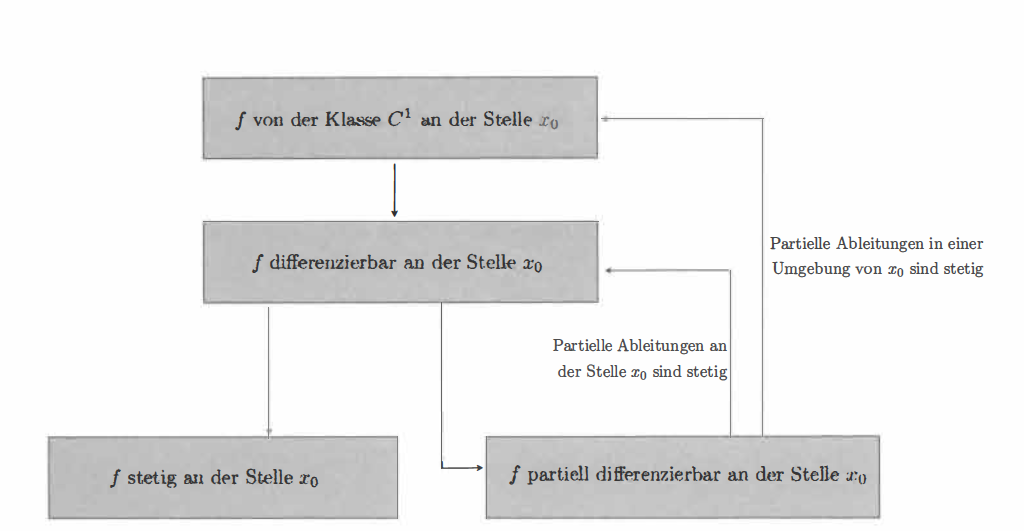
\includegraphics[width=8cm]{1}

\textbf{Prüfen, ob $f$ diffbar and $x_0$}:

$f$ stetig an $x_0$? Nein $\Rightarrow$ $f$ nicht diffbar.\\
$\Downarrow$ Ja\\
Ist $f$ in $x_0$ partiell diffbar, existiert $\frac{\partial f}{\partial x_i}(x_0)$? Nein $\Rightarrow$ $f$ nicht diffbar.\\
$\Downarrow$ Ja\\
Ist $\frac{\partial f}{\partial x_i}(x_0)$ stetig? Ja $\Rightarrow$ $f$ ist diffbar!\\
$\Downarrow$ Nein\\
Existiert eine lineare Abbildung $A$: $\mathbb{R}^n \rightarrow \mathbb{R}^m$ sodass $A=\nabla f(x_0)$, also existert:
\[
    \lim_{x\rightarrow x_0} \frac{|f(x)-f(x_0)-\nabla f(x_0) - (x-x_0)|}{||x-x_0||}
\]?
Ja $\Rightarrow$ $f$ ist diffbar!\\
Nein $\Rightarrow$ $f$ ist nicht diffbar.

\subsection{Beschränkt, Geschlossen, Kompakt}

\textbf{Beschränkt (bounded)} Falls $||x||$ beschränkt für alle $x \in M$.\\

\textbf{Geschlossen (closed)} Jede Folge $(x_n)$ mit $x_n \in M$ ist $\lim (x_n) \in M$.\\

\textbf{Kompakt (compact)} Falls beschränkt und geschlossen\\

\subsection{Partielle Ableitung (Partial Derivative)}

$f$: $\mathbb{R}^n \rightarrow \mathbb{R}$ an Stelle $a$ nach $x_i$

\[
    \lim_{h \rightarrow 0} \frac{f(a_1, ..., a_i + h, ..., a_n) - f(a_1, ..., a_i, ..., a_n)}{h} =: \frac{\partial f}{\partial x_i}(a)
\]

\textbf{Wichtig}: Alle anderen $x_i$ werden als konstante behandelt bei Ableitung.

TODO: Check script + check vorlesungsnotizen

TODO: regeln

\subsubsection{Gradient}

\[
    \nabla f =
        \begin{pmatrix}
            \frac{\partial f}{\partial x_1}\\
            \vdots\\
            \frac{\partial f}{\partial x_n}
        \end{pmatrix}
\]

Gradient eines Skalarfeldes: Richtung: Richtung des steilten Anstiegs; Betrag: Stärke des Anstiegs.\\

\textbf{Regeln} ($n \in \mathbb{N}$, $c$ konstant, $u, v$ Vektoren):
$\text{grad}(c) = 0$,
$\text{grad}(c \cdot u) = c \cdot \text{grad}(u)$ (Linearität),
$\text{grad}(u + v) = \text{grad}(u) + \text{grad}(u)$ (Addition),
$\text{grad}(u \cdot v) = \text{grad}(u) \cdot \text{grad}(u)$
(Produktregel),
TODO andere gradienten regeln von der übungsstunde 5
TODO Serie 5 2.1 senkrecht satz 
$\text{grad}(u^n) = n \cdot u^{n-1} \cdot \text{grad}(u)$ ($n\neq 0$).\\


\subsubsection{Richtungsableitung (Directional Derivative)}

\textbf{Rezept Richtungsableitung $D_u f(a)$} für $f$ in Richtung $u$ in Punkt $a$: 1) $u$ normieren: $\tilde{u} = \frac{u}{||u||}$ 2) Gradient $\nabla f(x)$ berechnen.

\[
    D_u f(a) = \tilde{u} \cdot \nabla f(a)
\]

\subsubsection{Hesse-Matrix (Hessian Matrix)}    

\[
    \text{Hess}(f) =
        \begin{pmatrix}
            \frac{\partial^2 f}{\partial x_1^2}&\hdots&\frac{\partial^2 f}{\partial x_1 x_n}\\
            \vdots&\ddots&\vdots\\
            \frac{\partial^2 f}{\partial x_n x_1}&\hdots&\frac{\partial^2 f}{\partial x_n^2}
        \end{pmatrix}
\]

\textbf{Trick Definitheit 2x2 Hessematrix:}

\[
    H =
        \begin{pmatrix}
            a_{11} & a_{12}\\
            a_{21} & a_{22}
        \end{pmatrix}
\]

Falls symmetrisch und und $\text{det}(H) > 0$:

$a_{11} > 0 \iff$ positiv definit;

$a_{11} < 0 \iff$ negativ definit;

sonst indefinit.

\subsubsection{Satz von Schwarz}

$f \in C^2$. Gilt nur für zwei und drei verschiedene Variablen. Beliebige Potenzen von $x_i$ und $x_j$ möglich.

\[
    \frac{\partial^2 f}{\partial x_i x_j} = \frac{\partial^2 f}{\partial x_j x_i} \forall i, j \in \{1, ..., n\}
\]

\subsubsection{Jakobimatrix (Jacobian Matrix)}

\[
    f(x, y) =
        \begin{pmatrix}
            f_1(x, y)\\
            \vdots\\
            f_n(x, y)
        \end{pmatrix}\ 
    \text{J}_f(x, y) =
        \begin{pmatrix}
                \frac{\partial f_1}{\partial x} & \frac{\partial f_1}{\partial y}\\
                \vdots&\vdots\\
            \frac{\partial f_n}{\partial x} & \frac{\partial f_n}{\partial y}
        \end{pmatrix}
\]

\subsection{Taylorpolynome}

\[
    f(x) = f(a) + f'(a)(x-a) + \frac{1}{2} f''(a)(x-a) + \frac{1}{3!} f^{(3)}(a)(x-a) + ...
\]

\textbf{Zwei Variablen}, $\Delta x = x - x_0$, $\Delta y = y - y_0$

\begin{align*}
    f(x, y) = f(x_0, y_0) &+ \frac{\partial f}{\partial x} \Delta x + \frac{\partial f}{\partial y} \Delta y\\
    &+ \frac{1}{2} \left(\frac{\partial^2 f}{\partial x^2} (\Delta x)^2 + 2\frac{\partial^2 f}{\partial x \partial y} \Delta x \Delta y + \frac{\partial^2 f}{\partial y^2} (\Delta y)^2\right)\\
    &+ \frac{1}{3!} \left(\frac{\partial^3 f}{\partial x^3} (\Delta x)^3 + 3\frac{\partial^3 f}{\partial x^2 \partial y} (\Delta x)^2 \Delta y + 3\frac{\partial^3 f}{\partial x \partial y^2} \Delta x (\Delta y)^2 + \frac{\partial^3 f}{\partial y^3} (\Delta y)^3\right)\\
    & + ...
\end{align*}

\textbf{Rezept Tangentialebene}: Tangentialebene in $P=(x_0, y_0, f(x_0, y_0))^T$ = Taylorpolynom 1. Ordnung in $x_0, y_0$.

\subsection{Change of variable}

Seien $x, y$ die alten Variablen und $u, v$ die neuen Variablen. Erstelle Abbildung $h:$ Neu $\to$ Alt, also $h: (u, v) \mapsto (x, y)$. Sei $f: (x, y) \to \mathbb{E}$, erstelle $g = f \circ h = h(f(x))$. $d (f \circ g) (x_0) = df(g(x_0)) \cdot dg(x_0)$

Übungsstunde 5: CHANGE OF VARIABLE?.??.? skript 3.6 TODO THIS

\subsection{Extremstellen}

\textbf{Rezept}: 1) Gradient berechnen 2) Gradient $=0$ setzen $\implies$ kritische Punkte. 3) Hessematrix berechnen 4) für jeden kritischen Punkt: Falls die Hessematrix positiv definit ist $\implies$ lokales Minimum; falls Hessematrix negativ definit ist $\implies$ lokales Maximum; sonst Sattelpunkt.\\

\textbf{Rezept für abgegrenzte Skalarfelder}: 1) Skalarfeld nach kritischen Punkten untersuchen 2) Alle Begrenzungen des Skalarfelder einzeln nach kritischen Punkten berechnen. Beispiel Dreieck: alle Seiten parametrisieren und alle Eckpunkte untersuchen.

\subsection{Lagrange Multiplikatoren}

Verfahren zur Lösung von Optimierungsproblemen mit Nebenbedingungen.

\subsection{Satz der Impliziten Funktion}

Ziel: Existenz von lokalen 

\subsection{Satz der Umkehrabbildung}